%% LyX 2.2.2 created this file.  For more info, see http://www.lyx.org/.
%% Do not edit unless you really know what you are doing.
%%%%%%%%%%%%%%%%%%%%%%%%%%%%%% User specified LaTeX commands.
%\usepackage{multirow}
%\usepackage{floatrow}

\documentclass[11pt]{article}%
\usepackage[latin9]{inputenc}
\usepackage{amsmath}
\usepackage{amssymb}
\usepackage[authoryear]{natbib}
\usepackage{float}
\usepackage{pdfpages}
\usepackage{graphicx}
\usepackage{amsfonts}
\usepackage{subcaption}
\usepackage{amsthm}
\usepackage{enumerate}
\usepackage{epsfig}
\usepackage{ifthen}
\usepackage{latexsym}
\usepackage{syntonly}
\usepackage{rotating}
\usepackage{lscape}
\usepackage{color}
\usepackage{booktabs}
\usepackage[bottom]{footmisc}
\usepackage{epstopdf}
\usepackage{makeidx}
\usepackage{xr}
% \usepackage{refcheck}%
\setcounter{MaxMatrixCols}{30}
%TCIDATA{OutputFilter=latex2.dll}
%TCIDATA{Version=5.50.0.2960}
%TCIDATA{CSTFile=LaTeX article (bright).cst}
%TCIDATA{LastRevised=Wednesday, August 16, 2023 19:55:35}
%TCIDATA{<META NAME="GraphicsSave" CONTENT="32">}
%TCIDATA{<META NAME="SaveForMode" CONTENT="1">}
%TCIDATA{BibliographyScheme=BibTeX}
%TCIDATA{Language=American English}
%BeginMSIPreambleData
\providecommand{\U}[1]{\protect\rule{.1in}{.1in}}
%EndMSIPreambleData
\textwidth=6.6in
\textheight=8.9in
\headheight=0.0in
\oddsidemargin=0.0in
\headsep=0.0in
\topmargin=0.0in
\newtheorem{theorem}{Theorem}
\newtheorem{corollary}{Corollary}
\newtheorem{case}{Case}
\newtheorem{lemma}{Lemma}
\newtheorem{proposition}{Proposition}
\newtheorem{assumption}{Assumption}
\theoremstyle{definition}
\newtheorem{definition}{Definition}
\newtheorem{example}{Example}
\newtheorem{remark}{Remark}
\def\baselinestretch{1.3}
\newcommand{\abs}[1]{\lvert#1\rvert}
\newcommand{\norm}[1]{\left\lVert#1\right\rVert}
\DeclareMathOperator*{\adjugate}{adj}
\DeclareMathOperator*{\sign}{sgn}
\allowdisplaybreaks
% \externaldocument{Wealth_effect_HARA_Supp_2022}






\begin{document}
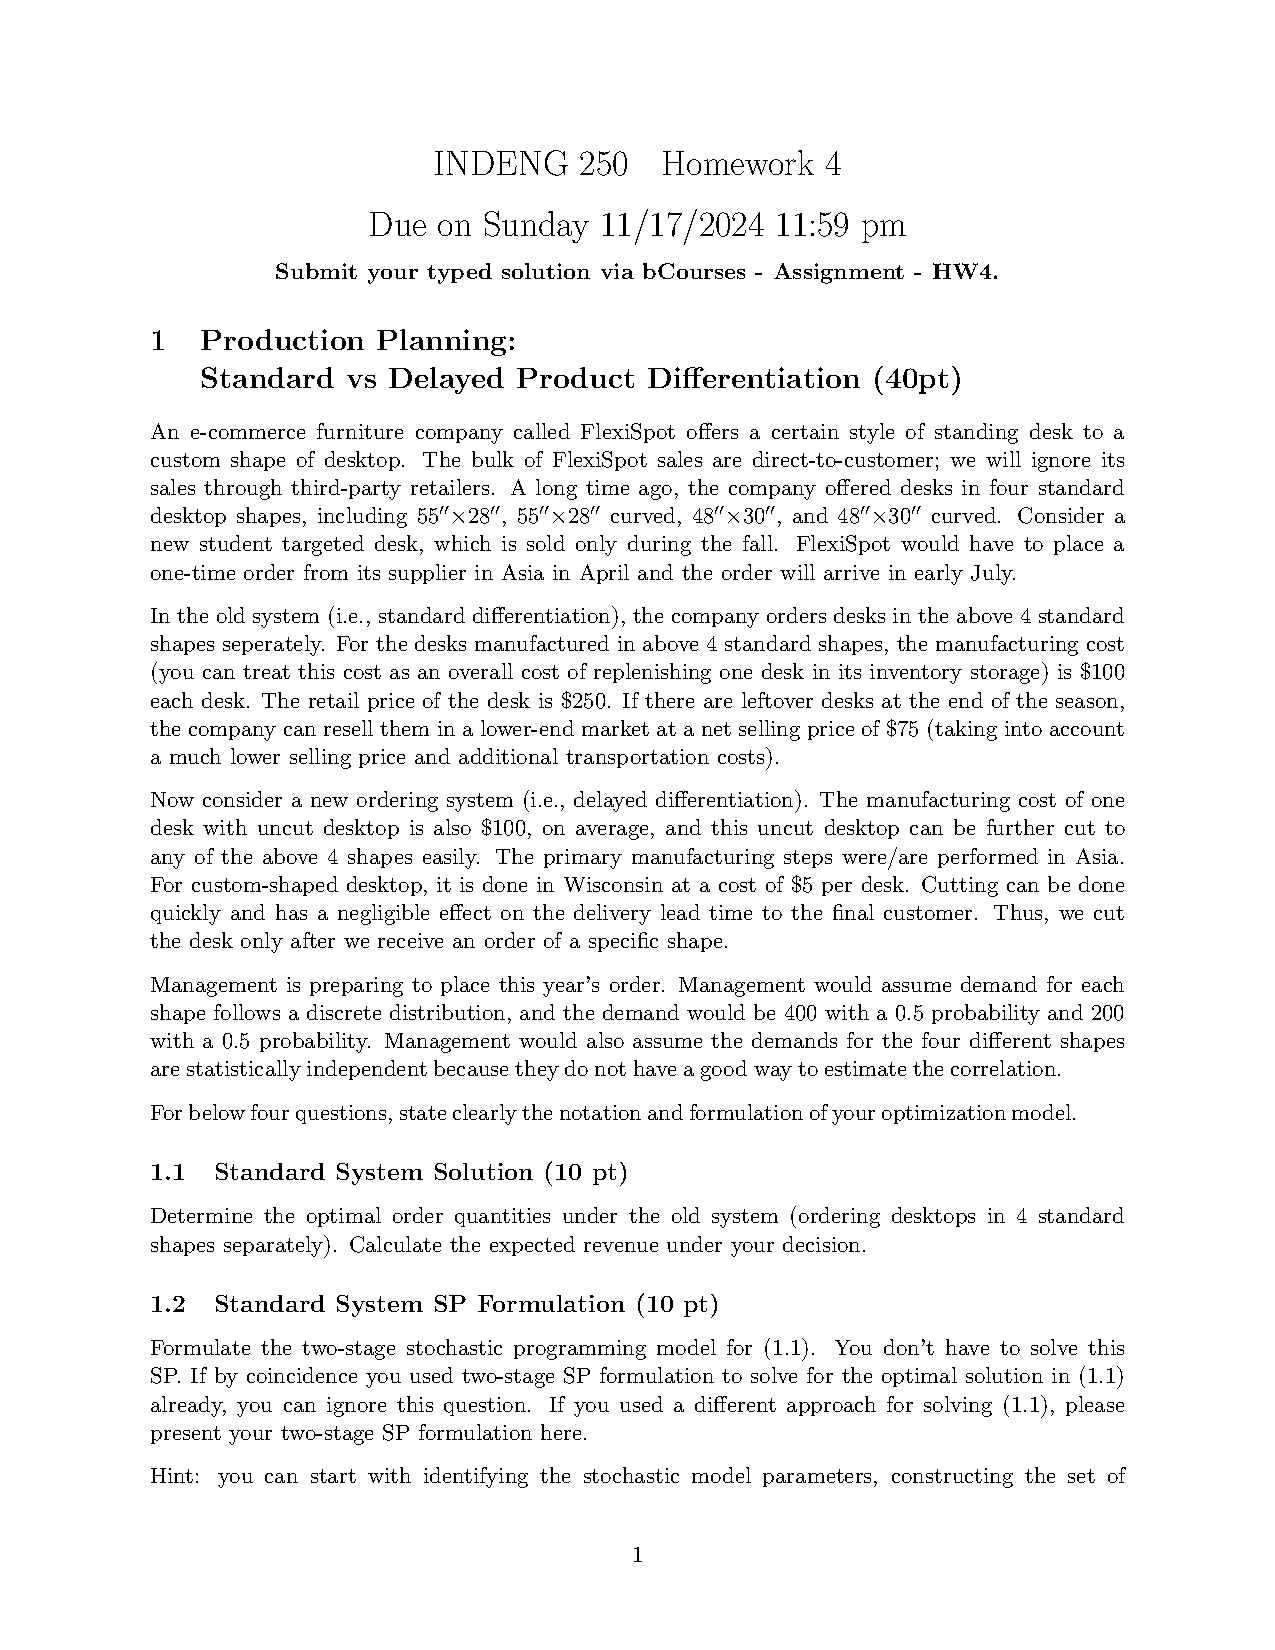
\includepdf[pages={1,2,3,4}]{homework_4.pdf}
\title{INDENG 250 PS4}
\author{Junyu Guo}
\date{\today }
\maketitle
\section{Problem 1}
1.1    
The demand for each shape with discrete probability. 
\begin{equation}
    P(D=200)=P(D=400) = 0.5.
\end{equation}
The demand for four shapes are statistically independent.
In the old system, we would order the four shapes separately, and we assume that we place an order with $x_i$ for each shape. Then the expectation of the whole revenue is 
\begin{equation}
    R = \sum_{i=1}^4 \mathbb{E}[-100 x_i+ 250\min(x_i,d_i)+75 (x_i-d_i)^+].
\end{equation}
Since each $d_i$ are uncorrelated, we can optimize for each $x_i$ separately.
\begin{equation}
    \max \mathbb{E}[-100 x_i+ 250\min(x_i,d_i)+75 (x_i-d_i)^+]=150 x_i-175(x_i-d_i)^+, d_i\sim \mathcal{D}_i. \label{separate reward}
    \end{equation}
    we consider the three cases
    \begin{itemize}
        \item $x\leq 200$. Then (\ref{separate reward}) can be formulated as 
        \begin{equation}
            \max 150x_i\leq 150*200=30000.
        \end{equation}
\item $200\leq x_i\leq 400$, we can rewrite (\ref{separate reward}) as 
\begin{equation}
    150x_i-0.5*175*(x-200)\leq 150*400-17500=42500.
\end{equation}
\item $x_i\geq 400$, then we can also have 
\begin{equation}
    175*300-25x_i\leq 52500-25*400=42500.
\end{equation}
    \end{itemize}
Therefore for each shape we should pick $x_i=400$, and the total quantity $x=\sum_i x_i=1600$. And the total revenue is $4*42500=170000$.    




1.2   

Now we formulate the 2-state stochastic programming model for (1.1)
\begin{equation}
    \begin{aligned}
        &\max g(x)+\mathbb{E}_{\xi}[Q(x,\xi)],\\
        \text{where}\quad  &g(x) =-100\sum_{i=1}^4 x_i, Q(x,\xi) = \sum_{i=1}^4 250(x_i,\xi_i)+75(x_i-\xi_i)^+.
    \end{aligned}
\end{equation}
  Here $x=(x_1,x_2,x_3,x_4)^\top$ is the decision variable, and $\xi=(\xi_1,\xi_2,\xi_3,\xi_4)$ is the uncertain data. 


  1.3     
  Now we only need to consider what is the total number of demand $d=\sum_i d_i$. Then we order $x$ from Asia and the whole revenue can be formulated as 
  \begin{equation}
      -100x -5\min(x,d)+250\min(x,d)+75(x-d)^+=145x-170(x-d)^+.
  \end{equation}
  $\mathbb{P}(d\leq x)=\frac{145}{170}=\frac{29}{34}$
  therefore we should choose $x=1400$ or $1600$, and compare the results.     
We should choose $x=1400$, and the total revenue is $166875$, which is smaller than 170000, therefore the company loses money by $3125$ from taking the new system.


  1.4 Now we formulate this problem as a two-state stochastic programming problem,
  \begin{equation}
      \begin{aligned}
      &  \max  g(x)+\mathbb{E}_\xi [Q(x,\xi)],\\
      & g(x) = -100x, Q(x,\xi) = -5\min(x,\xi)+250\min(x,xi)+75(x-\xi)^+
      \end{aligned},
  \end{equation}
  where $\frac{\xi-800}{200}\sim \operatorname{Binoal(4,0.5)}$.     


\section{Problem 2}
\subsection*{Problem Formulation}

We aim to maximize the total reward while managing vehicle delivery to two dealer sites. The variables and constraints are defined as follows:

\subsection*{Decision Variables}
\begin{itemize}
    \item \( K_{1t} \): Number of carriers moving from location \( I \) to dealer 1 on day \( t \).
    \item \( K_{2t} \): Number of carriers moving from location \( I \) to dealer 2 on day \( t \).
    \item \( K_{3t} \): Number of carriers moving from location \( I \) to dealer 1, and then to dealer 2 on day \( t \).
    \item \( y_{kjt} \): Number of vehicles unloaded at dealer \( j \) by carrier \( k \) on day \( t \).
    \item \( s_{jt} \): Inventory (unsold cars) at dealer \( j \) by the end of day \( t \).
\end{itemize}

\subsection*{Parameters}
\begin{itemize}
    \item \( d_{it} \): Demand of cars for dealer \( i \) on day \( t \).
    \item \( q \): Maximum number of vehicles a carrier can hold.
    \item \( c \): Transportation cost per mile for each carrier.
    \item \( h \): Holding cost per unsold car at the end of the day.
    \item \( d_{I1} \): Distance between location \( I \) and dealer 1.
    \item \( d_{I2} \): Distance between location \( I \) and dealer 2.
    \item \( d_{12} \): Distance between dealer 1 and dealer 2.
\end{itemize}

\subsection*{Objective Function}
\[
\max \sum_{t=1}^6 \Bigg[ \sum_{i=1}^2 -h (s_{it} - d_{it}) 
- c \Big( \sum_{k=1}^{K_{1t}} (d_{I1} + d_{I1}) 
+ \sum_{k=1}^{K_{2t}} (d_{I2} + d_{I2}) 
+ \sum_{k=1}^{K_{3t}} (d_{I1} + d_{12} + d_{I2}) \Big) \Bigg]
\]

\subsection*{Constraints}
\begin{enumerate}
    \item \textbf{Carrier Load Constraints:}
    \begin{align*}
        & y_{k1t} \leq q, \quad y_{k2t} = 0 \quad \forall k \in [K_{1t}] \\
        & y_{k2t} \leq q, \quad y_{k1t} = 0 \quad \forall k \in [K_{2t}] \\
        & y_{k1t} + y_{k2t} \leq q \quad \forall k \in [K_{3t}]
    \end{align*}
    \item \textbf{Demand Satisfaction:}
    \[
    s_{1t} + \sum_{k=1}^{K_{1t}} y_{k1t} + \sum_{k=1}^{K_{3t}} y_{k1t} \geq d_{1t} \quad \forall t
    \]
    \[
    s_{2t} + \sum_{k=1}^{K_{2t}} y_{k2t} + \sum_{k=1}^{K_{3t}} y_{k2t} \geq d_{2t} \quad \forall t
    \]
    \item \textbf{Inventory Dynamics:}
    \[
    s_{jt} = s_{j(t-1)} + \text{deliveries to dealer } j - d_{jt} \quad \forall j \in \{1, 2\}, \; t
    \]
    where \( s_{j0} = 0 \) (no initial inventory).
\end{enumerate}

\subsection*{2.2 Numerical experiments}


\subsubsection*{Optimal Objective Value}
The optimal objective value is: \textbf{\$42,600.0}

\subsubsection*{Daily Delivery Plan}
\begin{tabular}{@{}lcccccc@{}}
\toprule
\textbf{Day} & \textbf{ Dealer 1} & \textbf{Dealer 2} & \textbf{Both Dealers} & \textbf{To Dealer 1} & \textbf{To Dealer 2} & \textbf{Inventory} \\ 
\midrule
1 & 1.0 & 1.0 & 1.0 & 4.0 & 4.0 & (2.0, 2.0) \\
2 & 1.0 & 1.0 & 2.0 & 8.0 & 8.0 & (0.0, 0.0) \\
3 & 0.0 & 0.0 & 0.0 & 0.0 & 0.0 & (6.0, 6.0) \\
4 & 1.0 & 1.0 & 2.0 & 8.0 & 8.0 & (4.0, 4.0) \\
5 & 1.0 & 1.0 & 2.0 & 8.0 & 8.0 & (2.0, 2.0) \\
6 & 1.0 & 1.0 & 2.0 & 8.0 & 8.0 & (0.0, 0.0) \\
\bottomrule
\end{tabular}
And the code is demonstrated as follows.
\begin{figure}[H]
    \centering
    % First figure
    \begin{subfigure}[b]{0.45\textwidth}
        \centering
        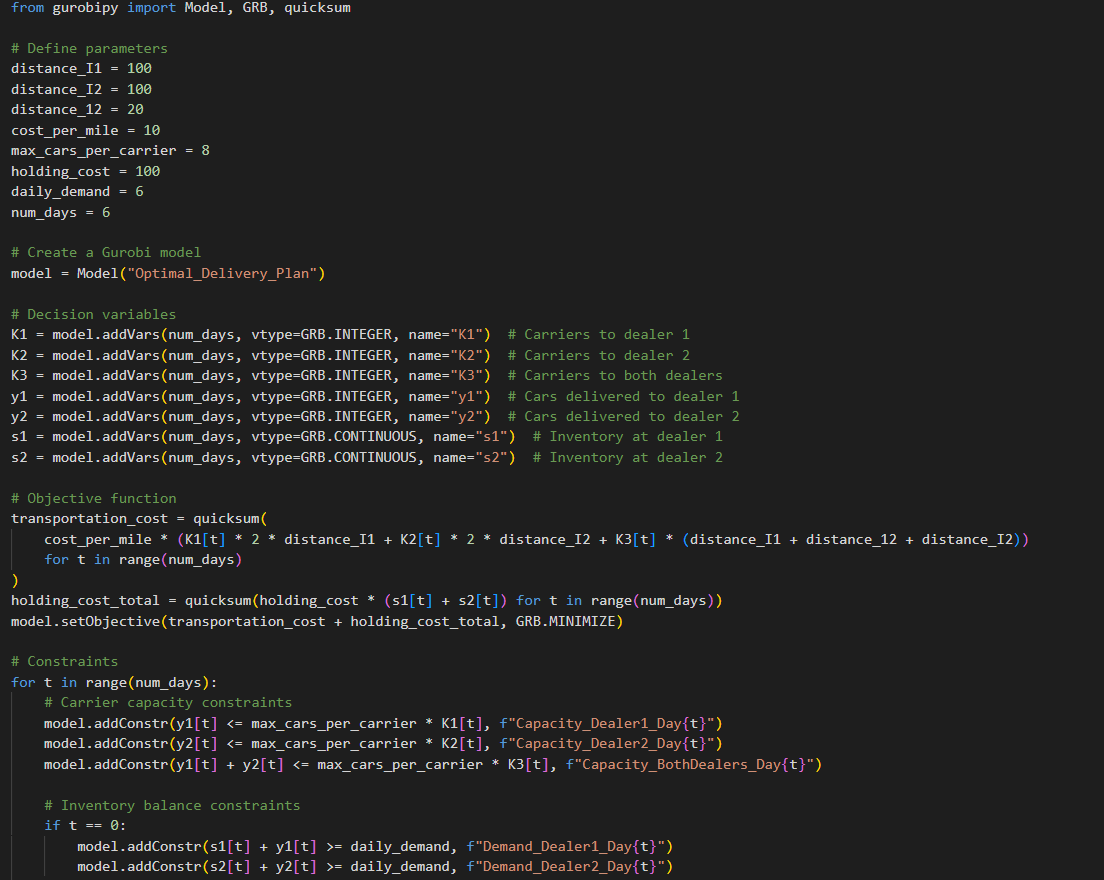
\includegraphics[width=\textwidth]{res1.png}
        \caption{Result 1: Optimal Delivery Plan Visualization}
        \label{fig:res1}
    \end{subfigure}
    % Second figure
    \begin{subfigure}[b]{0.45\textwidth}
        \centering
        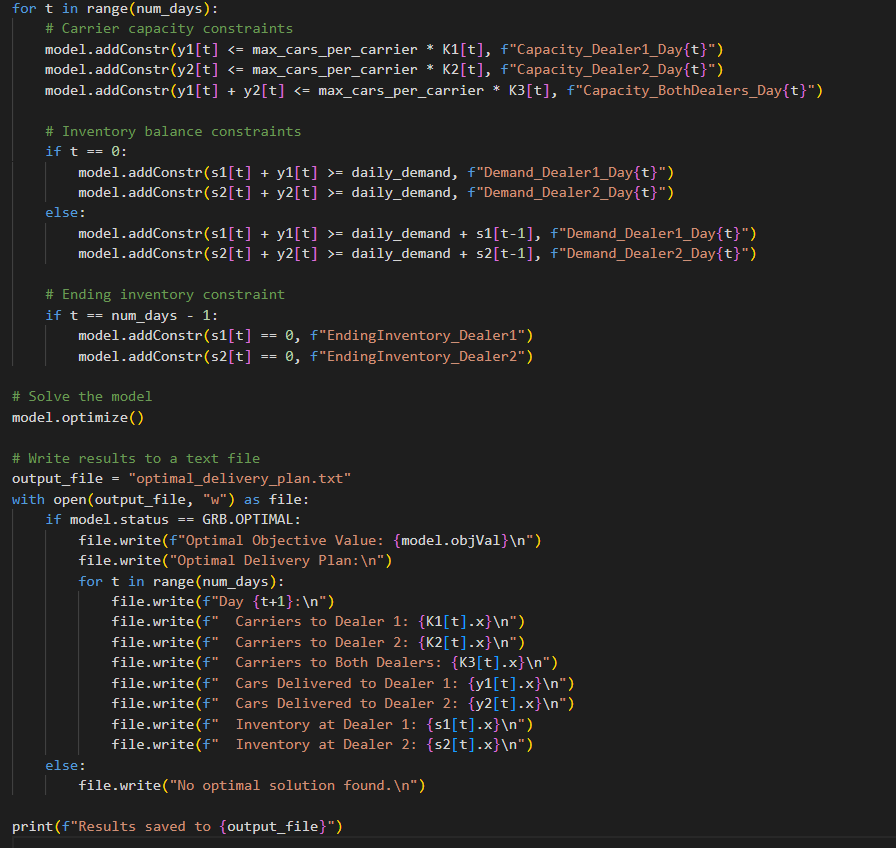
\includegraphics[width=\textwidth]{res2.png}
        \caption{Result 2: Inventory and Carrier Utilization}
        \label{fig:res2}
    \end{subfigure}
    \caption{Optimal Delivery Plan Results.}
    \label{fig:results}
\end{figure}

\subsection*{Interpretation of the Plan}
- On each day, the number of carriers and cars delivered to each dealer are listed along with the remaining inventory at the end of the day.
- The optimal delivery plan minimizes transportation and holding costs over the 6-day planning horizon.


  
\end{document}